\chapter{Fault detection in Utility Scale Photovoltaic Plants} \label{chap:chap2}


\section{Utility-Scale Photovoltaic System's Architecture}

Utility-scale photovoltaic (PV) power plants are large-scale systems connected to the electrical grid, having installed capacities ranging from kilowatts peak (kWp) to megawatts peak (MWp). These systems typically consist of many PV panels interconnected through power electronics to aggregate and inject power into the grid. The number and type of components in a PV power plant depend on the plant's scale and topology, with different configurations possible for large-scale applications, including central inverters, string inverters, and multi-string inverters \cite{lspv}. The physical installation of PV modules can include solar tracking apparatuses, such as single and dual-axis trackers \cite{Mourad2022}, which add to system complexity and change production behavior. Understanding the architecture and components of PV power plants is vital for designing, operating, and maintaining these systems, as it helps optimize their performance and reliability.

\begin{figure}[h!]
    \centering
    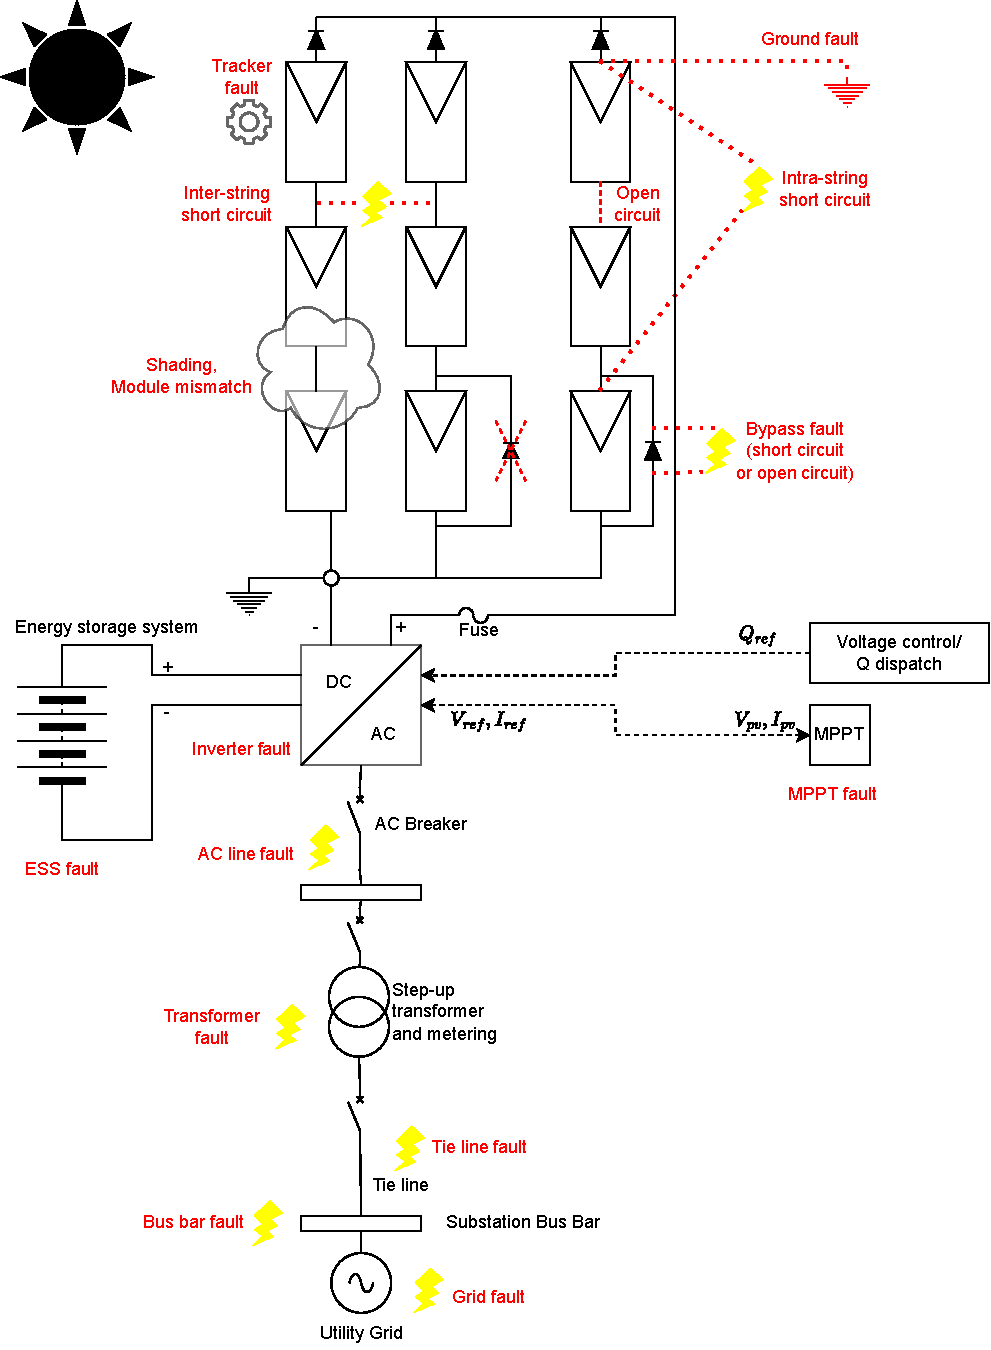
\includegraphics[width=15cm]{figures/chapter2/pvplant.drawio.pdf}
    \caption{Representation of utility-scale PV plant components and some possible faults.}
    \label{fig:topologies}
\end{figure}

Figure \ref{fig:topologies} presents a typical utility-scale PV plant architecture using the central inverter (or possibly multi-string inverter) configuration. It is noticeable that many system components may fail in one or more ways, which is why monitoring and fault detection algorithms are essential to maintain state estimation. The main subsystems considered in this work are the following:

\begin{itemize}
    \item Solar photovoltaic panels (with or without bypass diodes).
    \item Tracking mount.
    \item Electrical cabling.
    \item Inverter(s) (mostly with Max Power Point Trackers).
    \item AC Transformer(s).
    \item Protection components (circuit breakers, fuses, surge protectors,
    etc.)
\end{itemize}

Most of these components have intrinsic variables, such as voltage and current values, that can help determine their operation states. Given that the utility grids (and the associated electricity market) integrate large-scale PV assets, some of the before-mentioned components require constant monitoring and control, achieved with adequate embedded systems and sensor infrastructure \cite{AIPV}. Since monitoring utility-scale PV assets relies on the investment and technologies employed, engineers must consider data availability when developing data-driven algorithms. Thanks to the continuous advancements in communication technologies, namely in IoT (Internet Of Things), data acquisition is becoming faster, more reliable, and more precise. Not only is this fundamental for real-time asset assessment, but it also allows better training of fault detection algorithms. However, on the industrial scale (in the order of MWp production), having sensors embedded in every PV module comes with a high economic cost. Inverters are the components that usually possess monitoring capabilities, though the grid-tie connection should also be equipped with sensors. These can be considered the primary sources of information from utility-scale PV plants, with the most accurate, fast, and reliable data acquisition.

\begin{figure}[h!]
    \centering
    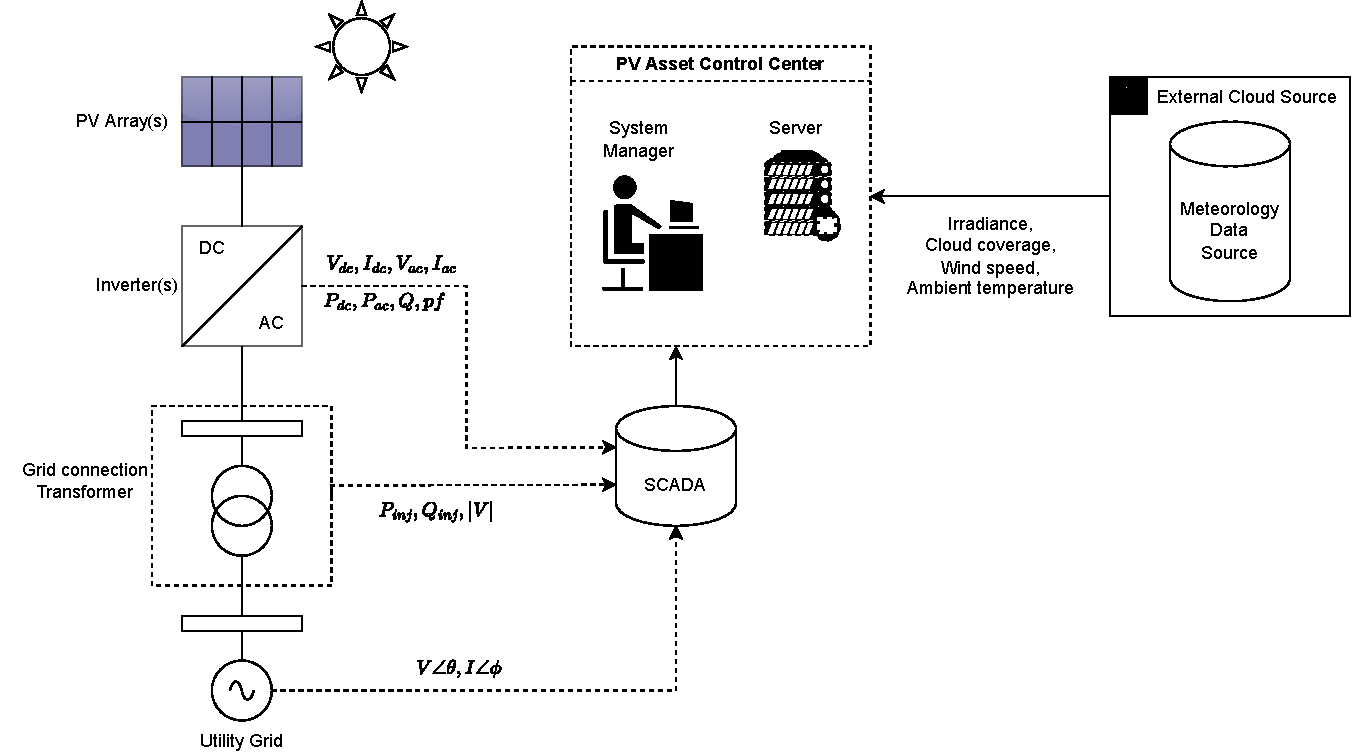
\includegraphics[width=\linewidth]{figures/chapter2/pvdata.drawio.pdf}
    \caption{Typical data flow of utility-scale PV power plants.}
    \label{fig:pvdataflow}
\end{figure}

Figure \ref{fig:pvdataflow} represents a simplified data flow representation of a grid-tied PV system's most commonly available state variables, with most of them suggested by the IEC 61724 norm \cite{iec61724}. An external meteorological data source is defined since the PV system manager usually needs climate information for (at least) forecasting purposes.


\section{Faults in Photovoltaic Systems}

Several types of faults can occur in utility-scale photovoltaic (PV) power plants (figure \ref{fig:topologies}), which can negatively impact the performance and reliability of the system, possibly causing safety hazards \cite{Alam2015}. Some are challenging to detect and protect the electrical installation against, thus requiring sophisticated detection algorithms \cite{Pillai2018}. According to \cite{Pillai2018}, these faults can fit into three categories: electrical, mechanical, and environmental. Electrical faults include short circuits, open circuits, and inverter failure, affecting the PV panels' power output and the system's overall efficiency. Mechanical faults include broken panels, damaged cables, and defective inverters, which can lead to system downtime and reduced performance. Environmental faults include extreme weather events, such as hail or strong winds, which can damage the PV panels and other components \cite{faults}. Figure \ref{fig:faults} illustrates a more extensive summary of fault types. A comprehensive literature review on most types of faults is covered by 

Although also prone to failure, most literature on fault detection and classification for photovoltaic systems does not encompass solar tracking faults: most studies cover fixed PV systems. The supervision of these subsystems can either be sensor-based \cite{Stepanov2014} or image-based, and some authors developed fault detection methods for these apparatuses \cite{Amaral2021}, using image processing on aerial photography to determine modules' slopes. This category of failures could be better supported when developing electrical data-driven algorithms since they can significantly affect the system's efficiency. Thus, this work will attempt to include this fault category in the proposed fault detection methodology.

\begin{figure}[h]
    \centering
    \includegraphics[width=16cm, trim={2cm 2.1cm 2cm 12cm},
    clip]{figures/chapter2/types\_of\_faults.pdf} \caption{"Classification of
    faults in PV Systems".} Image source and copyright: \cite{Pillai2018}.
    \label{fig:faults}
\end{figure}

Throughout the literature \cite{Braun2011}, some of the most studied faults in the context of fault detection are:

\begin{itemize}
    \item Shading: partial coverage, temporary or not, of a PV array or module. It might result in a Hot Spot fault.
    \item Soiling: dirt accumulation, blocking sunlight from reaching PV Cells. It might also result in a Hot Spot fault.
    \item Short circuit: either line-line or line-ground.
    \item Open circuit: connection breakage between modules.
    \item DC arc fault: electricity plasma arc formed on broken connections.
\end{itemize}

According to a 2017 survey conducted on five utility-scale PV plants in Italy, the authors observed failure rates from
<1\% to 3\% in the majority of plants, and 81.8\% on the worst scenario \cite{Grimaccia2017}. The high failure rate of
the latter had a demonstrated cause that originated from manufacturing mistakes: snail trails. Besides this phenomenon,
hot spot faults and bypass diode faults/disconnections were among the most common.

Alongside manufacturing failures, installation, planning, and other external effects can be the root cause for many of the presented faults \cite{sunny}.

\begin{figure}[h]
    \centering
    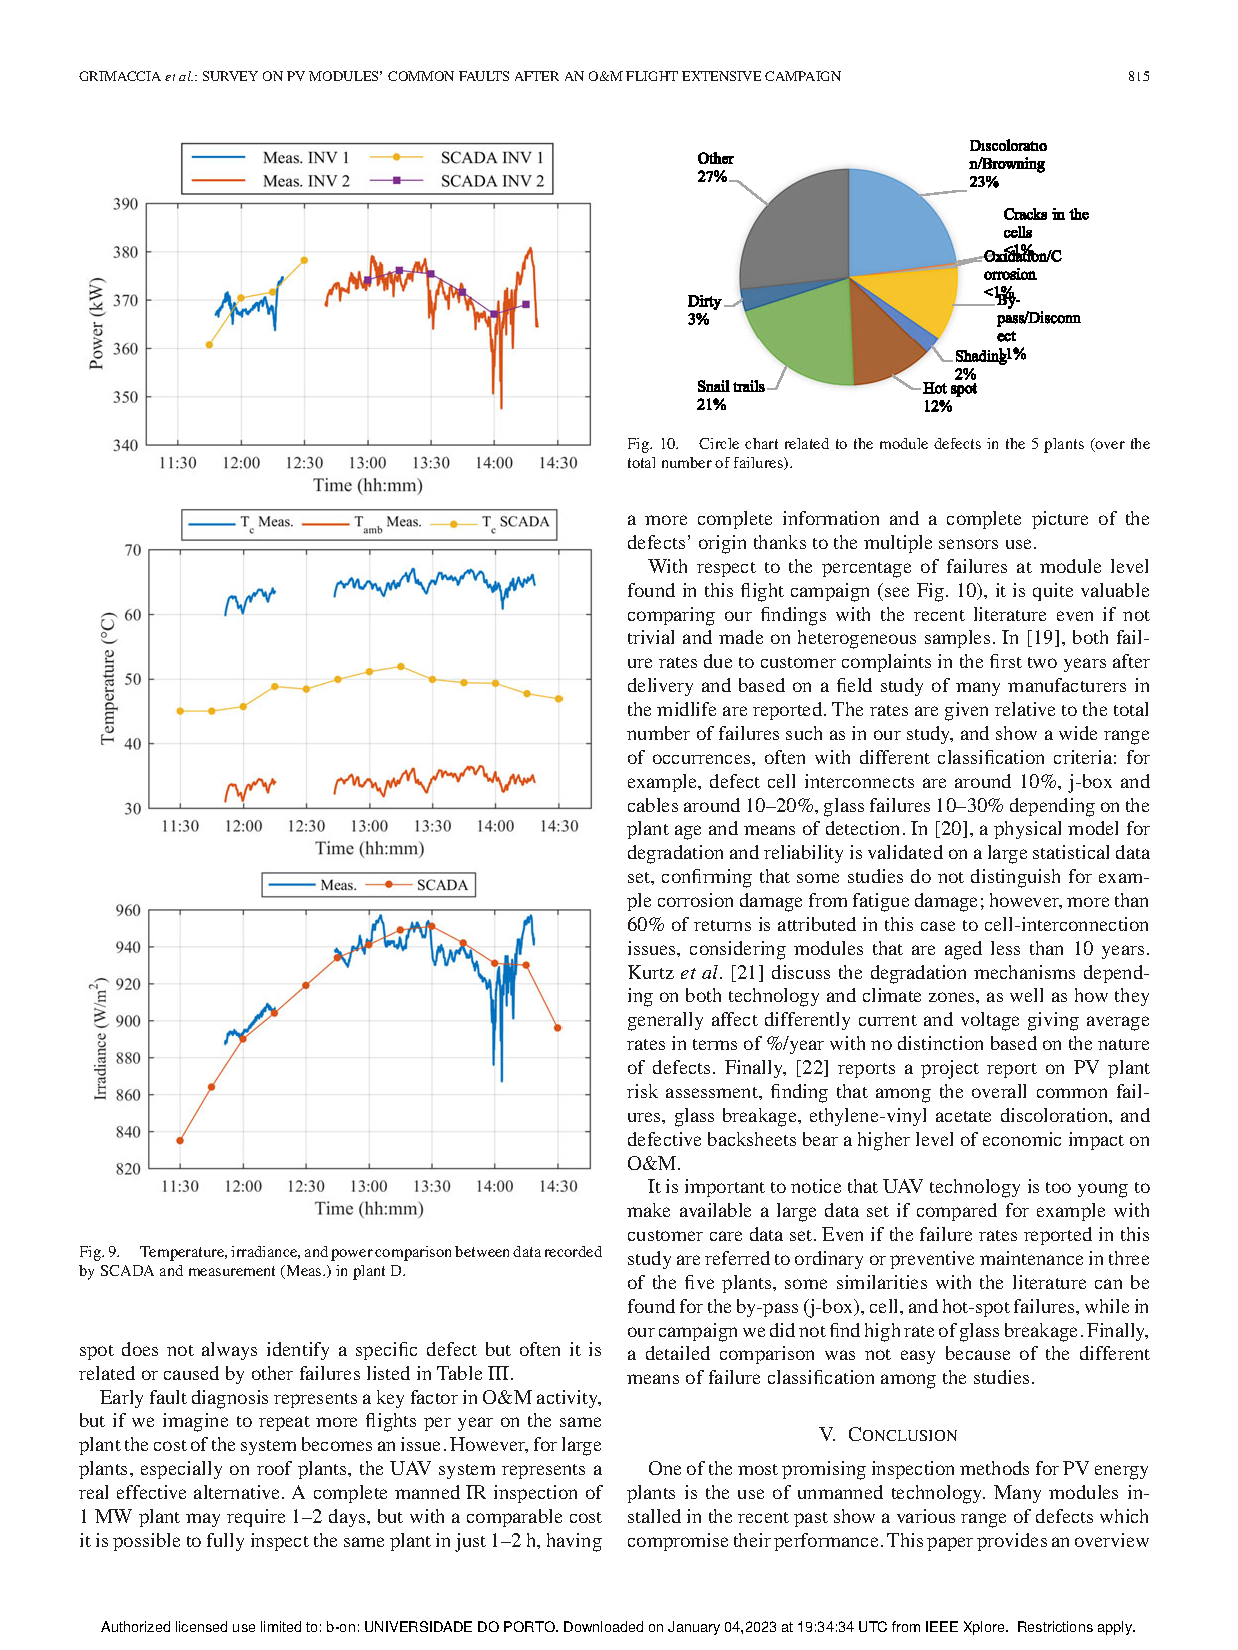
\includegraphics[width=10cm, trim={11cm 20.6cm 2.4cm 2cm},
    clip]{figures/chapter2/chartfailsurvey.pdf} \caption{"Circle chart related to the module defects in the 5 plants
    (over the total number of failures)."} Image source and copyright: \cite{Grimaccia2017}.
    \label{fig:faultchart}
\end{figure}

Having the distribution of fault types from real-life scenarios is quite helpful for formulating fault detection algorithms. It allows for better generation/selection of training data and decision of classes. In figure \ref{fig:faultchart}, it is possible to observe the failure type distribution for 24.254 inspected modules. Soiling, shading, and mechanically related failures were not as prominent, with only a group share of around 6\%. It is relevant to note that discoloration represents almost a quarter of all faults.

Although the study had a limited geographic scope, with only a few power plants diagnosed, it allows for a more realistic view of the common scenarios encountered in typical operational ground-mounted utility-scale PV power plants.

Due to the difficulty of classifying some of these faults, given their similarity on the consequent effect in the system, it will be seen in further sections that most fault detection algorithms only endeavor to classify between two to five types of reviewed faults.

\section{Modeling photovoltaic's physical/electrical behavior}

Photovoltaic cells are the fundamental components of photovoltaic panels. They are made from semiconductor materials, such as silicon,  and absorb photons that generate an electric current. Their electrical behavior is characterizable using the current-voltage (I-V) equation \ref{eq:iv}. This equation, which represents a fundamental relationship governing the operation of PV cells, can be used to predict their performance under various operating conditions, such as solar irradiance and temperature.

\begin{equation} \label{eq:iv}
    I = I_{ph} - I_d \times (e^{\frac{q \times (V_{pv} + I_{pv} \times R_{s})}{n \times k \times T}} - 1) - \frac{V_{pv} + I_{pv} \times R_s}{R_p}
\end{equation}

$I_{ph}$ (A) is the light-generated current;
$I_{0}$ (A) is the reverse saturation current;
$V_{pv}$ is the module's terminal voltage;
$I_{pv}$ is the module's output current;
$R_{s}$ ($\Omega$) is the series resistance;
$R_{p}$ ($\Omega$) is the shunt resistance;
$n$ (adimensional) is the diode ideality factor;
$k$ (J/K) is the Boltzman constant;
$T$ (K) is the cell temperature;
$q$ (C) is the electron charge;

For state estimation, it is crucial to accurately model PV modules' performance from the DC side of power converters. This information is vital for designing and optimizing PV power systems, as it enables predicting PV module performance under different conditions, as mentioned before. Accurate PV module models are also essential for state estimation and fault detection, as they provide critical information about the health and performance of PV modules, allowing for early identification of potential issues. In addition, they can be used to optimize the control and operation of PV power systems, which can improve the overall efficiency and reliability of the system \cite{Braun2011}.

Physical and empirical models broadly categorize the several state-of-the-art methods for modeling photovoltaic modules \cite{Braun2011}. Physical models lie on the fundamental physical principles governing PV modules' operation. They typically require detailed knowledge of the PV module's electrical and optical properties, such as its current-voltage (I-V) characteristics, spectral response, and temperature dependence. These models can accurately predict the PV module's performance under a wide range of operating conditions, but they may be complex and computationally intensive to implement \cite{Kumar2019}. On the other hand, empirical models are based on experimental data and are typically more straightforward to implement. However, they may not be as accurate as physical models, especially under conditions that differ significantly from those used to generate the experimental data (usually STC) \cite{Braun2011}. Some examples of state-of-the-art physical models for PV modules include the single-diode model (also known as the five-parameter model), and the two-diode model \cite{Godina2017}. In contrast, one of the most used state-of-the-art empirical models is the Sandia model \cite{Braun2011}. The choice of modeling method will depend on the specific application and the required level of accuracy and complexity; in some cases, there can be a combination of physical and empirical models.

Suppose the need arises to model PV modules in this work. In that case, it is critical to select a simple methodology so that the module's datasheet characteristics are sufficient to model the PV arrays accurately. In the case of utility-scale PV systems, detailed knowledge of the module's electrical and optical properties of empirical data may be limited, and building a model is only possible by using datasheet data. A complex model that requires more detailed information may not be feasible in such cases, and a simpler model that relies on fewer input parameters is more appropriate. The single-diode model seems appropriate for this use case, given the excellent trade-off between complexity and accuracy.

\subsection{The five-parameter model}

Figure \ref{fig:onediodedraw} presents the single-diode model representation of the photovoltaic module. According to the five-parameter model, the unknown parameters are determined by fitting the model to experimental data or using data from the PV module's datasheet. The single-diode model can predict the PV module's performance under a wide range of operating conditions while maintaining reasonable accuracy. However, remembering that the single-diode model is a simplified representation of the PV module, it will have poor accuracy under certain situations compared to the more representative two-diode model \cite{Godina2017}.

\begin{figure}[h]
    \centering
    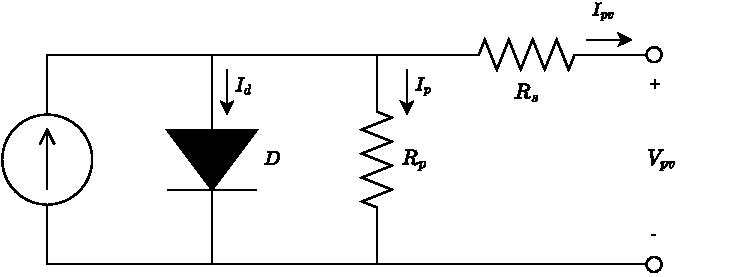
\includegraphics[width=10cm]{figures/chapter2/onediode.drawio.pdf} \caption{Single-diode model for photovoltaic modules.}
    \label{fig:onediodedraw}
\end{figure}

\section{Literature on Fault Detection and Classification for Photovoltaic Systems}

The parent field of fault detection is anomaly detection (also known as outlier detection), a highly studied subject in the scope of statistics \cite{Prasad2009}, applied in many scientific areas. Classification is also a well-studied subject in this field, with applications in numerous scientific contexts, from medical diagnosis to airport safety \cite{classification}. Consequently, usage or adaptations of generic tools and ad hoc methodologies have originated to aid in solving fault detection and classification problems in photovoltaics.

According to \cite{AIPV}, the tools dedicated to PV fault detection and state estimation mostly come from mathematical/statistical methodologies, machine learning, and deep learning applications. Regarding the three general problem-solving principles mentioned before, it's known that machine learning and deep learning are the most popular and successful ones for recent applications that ought to solve complex problems. However, this categorization is somewhat limited, with other literature suggesting an abundance of developed methodologies from different backgrounds, thoroughly reviewed in \cite{Hong2022} and \cite{Livera2019}. In \cite{Hong2022}, the authors consider two principal fault detection and classification algorithm branches: image-based and electrical-based. Image-based refers to aerial or visual capture of the PV array by photography and thermal imaging, commonly used along with artificial intelligence algorithms for assessing the photovoltaic module's state. Although the contribution and importance of such methods are appreciable, this work will mainly focus on the electrical-based ones, as the use case of the developed tool is bound to this type of data.

Electrical-based fault detection and classification algorithms come in many forms, ranging from more straightforward and focused on physical behavior to more abstract and data-driven. Since the proposed work might result in a hybrid approach, it is best not to discard algorithms entirely based on their solo importance.

% list methods

The developed tool in this work must meet certain real-life constraints, such as data availability, frequency, and accuracy. Therefore, the qualitative potential estimation for each methodology is based on the capability of adapting the proposed algorithm to the same restrictions. This evaluation process confines the methodology review to emphasize the ones thought to be most capable of implementation in a real scenario.


\subsection{Statistical and Signal Processing Algorithms}

Statistical methodologies look into historical data to find the characteristics of how samples relate to the population (interpolation). These methodologies yield good results in case studies of PV farms that have been logging data for a considerable time, suffering in the cases that do not. Therefore, they are limited in that it is required to have curated data sets of historical significance for relevant features of the studied systems.

Some algorithms consider incoming data from PV systems as signals, allowing the adaptation of signal processing theory to develop ad hoc algorithms. In \cite{Fan2020}, the authors successfully formulated a graph signal processing algorithm for fault classification that yields increasingly better results when there is a considerable amount of labeled data. The results outperformed other standard machine learning methods for the same training data, given 30\% or more of labeled data. On another note, the data utilized came from the PVWatts \cite{Dobos2013} dataset, and the PV system is on a small scale possessing a monitoring density and capability that should be considered irrealistic on a utility-scale. This same dataset appears in other mentioned references.

Notably, some graph-based methods for this purpose don't rely on signal processing theory. Section \ref{subsec:machinelearning} reviews these.

Coming up with a relatively simple algorithm, the authors in \cite{Iles2021} propose a power-based fault detection method that only requires delayed samples of the PV array's power output and a threshold. It is based on the fact that the power output of PV systems can't vary beyond a given point, considering a very short-term period (milliseconds). Although the simplicity and ease of implementation, it's clear that the success of this method requires feeding the algorithm with high-frequency data, which would only be feasible on-site (and with specialized equipment).

The literature on statistical and signal processing fault detection algorithms for PV is mostly quite dated (\cite{Buddha2012}, \cite{Zhao2014}, \cite{Vergura2008}), given that more recent machine learning methods have become increasingly attractive in this matter. Nonetheless, anomaly (or outlier) detection statistical algorithms can be used for fault detection in PV systems by identifying unusual patterns or deviations from normal behavior in the data collected from the PV system. Distance-based methods, such as Euclidean, Mahalanobis, and MCD-based distances \cite{Braun2011}, may be adequate. Although simple, these techniques might only work for detecting outliers in the context of PV systems if they are scale-invariant (due to the different magnitude in the system's state variables) and resilient to outlier contamination (only with MCD-based distance).

In \cite{Vergura2008}, the authors applied Analysis of Variance (ANOVA) and Kruskal-Wallis test for inverter failure detection, with the downside of only being able to identify outliers in a sub-array resolution, i.e., not for specific string or module failures.

\subsection{Machine Learning Algorithms} \label{subsec:machinelearning}

Machine learning came to solve some of the complications referred to in the two past subjects, as neural networks (or other learning structures) are easily capable of modeling complex, non-trivial, and nonlinear relations between data. Still, they are as good as the training data, with many structures requiring many representative learning examples to achieve good results. Their output can also be very obfuscated, meaning that many methods do not allow a direct interpretation of the relationship between inputs and outputs. This "black-box" characteristic, specifically of neural networks, is considered a disadvantage. Besides, extrapolating data remains a challenge when classically using these structures. Still, they have immense applications for PV systems, from MPP (Max Power Point) estimation to power forecasting, soiling, and fault prediction.

FALTA MENCIONAR O ESTADO DA ARTE DESTA SECÇÃO.

\subsection{Deep Learning Algorithms}

The field of deep learning branches off from machine learning, with the term "deep" referring to amplified machine learning structures that ought to understand data patterns through numerous intertwined neuron connections. A simple example of a deep learning model would be the design of an artificial neural network with multiple hidden layers (multidimensional), with the intuition that each of these "extra" layers achieves feature/pattern recognition in a cascade. They have been explored alongside machine learning techniques for PV fault detection, although the known disadvantage is a usually high computational cost and relatively tricky implementation.

FALTA MENCIONAR O ESTADO DA ARTE DESTA SECÇÃO.

While classical fault detection lies in the synchronous and direct evaluation of state estimation variables, fault prediction requires the input of time-series features. Although relatively simple, some classical time-series forecasting and analysis tools can be of great support to help design a fault prediction algorithm, such as Box-Jenkins methods and the Partial Auto-correlation function. Still, the majority of modern prediction tools comprise neural networks and variations. With this in mind, recent developments in the intelligent composition of learner structures spark some interest in the application to this field, such as the new deep learning technique named Cell Complex Neural Networks \cite{Hajij2020}. Further investigation of such modern practices will unroll throughout the development of this work.


\subsection{Proposed method's scope}

The proposed method should pertain to the hybrid category, with a central component of deep learning.